\documentclass[9pt,a4paper,oneside]{extbook}
\doublespacing
% Packages
% Packages

% Language-related

\usepackage{setspace}
\usepackage[T1,T2A]{fontenc}
\usepackage[utf8]{inputenc}
\usepackage[english,bulgarian]{babel}

% Others
\usepackage{indentfirst}
\usepackage{amsmath}
\usepackage{blindtext} % Needed for creating dummy text passages
\usepackage[colorlinks=true,breaklinks,english]{hyperref}
\usepackage[hyphenbreaks]{breakurl}
\usepackage{xcolor}
\usepackage{ragged2e}
\definecolor{c1}{rgb}{0,0,0} % Blue
\definecolor{c2}{rgb}{0,0.3,0.9} % Light blue
\definecolor{c3}{rgb}{0.3,0,0.9} % Red blue
\hypersetup{
    linkcolor={c1}, % Internal links
    citecolor={c2}, % Citations
    urlcolor={c3} % External links/URLs
}

%\usepackage{cite} % Needed for cite

% Needed for cite and abbrvnat bibliography style
\usepackage[round,authoryear]{natbib}

% Needed for displaying bibliography and other in the table of contents
\usepackage[nottoc]{tocbibind}

\usepackage{graphicx} % Needed for \includegraphics
\usepackage{epstopdf}
\usepackage{longtable} % Needed for long tables over pages
\usepackage{bigstrut} % Needed for the command \bigstrut
\usepackage{enumerate} % Needed for some options in enumerate
\usepackage{todonotes} % Needed for todos
\usepackage{makeidx} % Needed for creating an index
\makeindex


% Page settings
% Page settings

% Needed for page border settings
\usepackage[top=1.8cm, bottom=1.8cm,left=2.0cm,right=2.0cm]{geometry}

% For writing with hyphenless justification (tries to)
\sloppy

\hyphenation{}
\hyphenpenalty=10000
\exhyphenpenalty=10000


% Custom commands

% This file defines some macros

% Text-bold-italic (makes the text bold and italic)
\newcommand{\tbi}[1]{\textbf{\textit{#1}}}

% Underline and italic
\newcommand{\imp}[1]{\underline{\textit{#1}}}


\begin{document}

\pagestyle{empty}
\begin{titlepage}

\center % Center everything on the page

\vspace{5mm}
\textsc{\Large Технологично училище Електронни системи към Технически
  университет - София}\\[0.5cm] % TUES ftw

\vspace{30mm}

{\Large \bfseries ДИПЛОМНА РАБОТА}\\[2cm]

\Large Тема: Мрежов анализатор с възможност за отдалечен анализ посредством
AngularJS 2 клиент

\vspace{40mm}

\begin{minipage}{0.35\textwidth}
\begin{flushright} \normalsize
Дипломант: \\[5mm]
Научен ръководител: \\[5mm]
\end{flushright}
\end{minipage}
~
\begin{minipage}{0.55\textwidth}
\begin{flushleft} \normalsize
Ивайло Арнаудов \\[5mm]
Стоил Стоилов\\[5mm]
\end{flushleft}
\end{minipage}\\[2cm]

{\normalsize София, $2017$} \\[0cm]


\vfill % Fill the rest of the page with whitespace

% List of symbols (kept just in case so far)

\newpage
\begin{flushleft}
\begin{Large}
\emph{\bf Списък на означения}\\
\end{Large}
\end{flushleft}
\begin{spacing}{1.241}
\vspace{10mm}
\begin{minipage}{0.2\textwidth}
\begin{flushleft} \normalsize
\ensuremath{\sigma_{y}(\tau)}\\
\end{flushleft}
\end{minipage}
~
\begin{minipage}{0.5\textwidth}
\begin{flushleft} \normalsize
Exponential regression function\\
\end{flushleft}
\end{minipage}\\[4cm]
\end{spacing}
\vfill

% List of abbreviations

\newpage
\begin{flushleft}
\begin{Large}
\emph{\bf Списък на съкращения}\\
\end{Large}
\end{flushleft}
\begin{spacing}{1.241}
\vspace{10mm}
\begin{minipage}{0.2\textwidth}
\begin{flushleft} \normalsize
VPN\\
\end{flushleft}
\end{minipage}
~
\begin{minipage}{0.5\textwidth}
\begin{flushleft} \normalsize
Virtual Private Network\\
\end{flushleft}
\end{minipage}\\[4cm]
\end{spacing}
\vfill

\pagestyle{plain}
%\listoftodos

\tableofcontents
\vfill

\setcounter{chapter}{-1}
\chapter{Увод}
\onehalfspacing
\pagestyle{fancy}
\fancyhf{}
\fancyhead[OC]{\leftmark}
\fancyhead[EC]{\rightmark}
%\renewcommand{\footrulewidth}{1pt}
\cfoot{\thepage}

\section{Компютърни мрежи}
\justify
Всеки от последните три века бива доминиран от някаква нова технология. Пример
за това е ерата на механичните системи съпътстващи Индустриалната революция през
XVIII век. За XIX век пък е характерен парния двигател. През XX век, ключовата
технология е събирането, обработката и дистрибуцията на информация. С развитието
й човечеството става свидетел на инсталацията на глобални телефонни мрежи,
изобретяването на радиото и телевизията, експоненциалния растеж на развитието на
компютърната индустрия и, разбира се, Интернет. Като резултат от огромния
технологичен прогрес в сферата на информационните технологии, през XXIв.
разликите между съхраняване, транспортиране и обработка на информация изтъняват,
а успоредно с това растат и изискванията на крайния потребител към
комуникационните услуги.

Въпреки крехката възраст на компютърната индустрия (напр. в сравнение с
автомобилната), тя прави значителен прогрес. През първите две десетилетия от
съществуването им, компютърните системи са били силно централизирани.
Университет или средно голяма фирма биха имали един или два компютъра, а
по-големите институции - по няколко. Идеята за съществуването на малки
устройства тип смартфон, които са взаимносвързани, е била по-скоро утопична.

Обединяването на компютрите и комуникациите оказва голямо влияние върху
организацията на самите компютърни системи. Старият модел при който един
компютър изпълнява заявките на цялата организация бива заменен от нов модел при
който голямо количество отделни, но взаимносвързани компютри извършват обработка
на дадена информация. Тези системи се наричат \textbf{компютърни мрежи}.
Неформална дефиниция за компютърна мрежа е множество от автономни компютри,
взаимносвързани (можещи да обменят информация помежду си) от една технология.

\section{Приложения на компютърните мрежи}

\subsection{Приложения на компютърните мрежи в бизнесa}

Обикновено повечето компании имат голямо количество компютри, най-често по един
за всеки служител. Изначално, те биха могли да работят в изолация един от друг,
но в даден момент идва необходимост те да бъдат свързани с цел служителите да
извършват работата си по-пълноценно чрез колаборация помежду си.

Един от основните проблеми, който решават компютърните мрежи е
\textbf{споделянето на ресурси}. Целта е информацията да бъде достъпна от всеки
в мрежата независимо от физическото му местоположение. Пример за това е група
служители на организация, използващи един общ принтер --- нито един от тях няма
нужда от личен такъв, затова и решението е по-евтино, бързо и по-лесно за
поддръжка от поддръжката на голямо количество принтери.

Дори по-важен проблем, който решават компютърните мрежи е споделянето на
информация. Малките и средни компании са фундаментално зависими от дигиталната
информация. Повечето компании имат записи за клиенти, за продукти, финансова
информация и т.н. онлайн. По-малките компании са традиционно разположени в един
офис, докато при по-големите интернационални компании компютрите и служителите
са разпрострени в много държави. Това обикновено бива имплементирано чрез
\textbf{Virtual Private Network (VPN)} с цел агрегация на
индивидуалните мрежи на различни местоположения в една обща.

В допълнение, компютърните мрежи дават възможността да се използват вече
изградената мрежова инфраструктура за телефонни разговори благодарение на 
технологията \textbf{Internet Protocol (IP) телефония}, или още известна като
\textbf{Voice over IP (VoIP)}. Те също предоставят механизми за по-богати
форми на виртуална комуникация -- споделяне на екрана (\textbf{Desktop sharing}),
видеоконференции, споделена обработка на документи, дори отдалечен мониторинг
на пациенти. Компютърните мрежи отварят вратите и за нов бизнес модел, наречен
електронна търговия (или \textbf{e-commerce}), който се развива с големи темпове в
последните години и става де факто стандард при търговията от всякакъв тип.

\subsection{Приложения на компютърните мрежи у дома}

В началото на компютърната индустрия причините за покупка на компютър от крайния
потребител са се свеждали до нужда от обработка на текст и игри. През XXI век,
най-голямата причина човек да се сдобие с персонален компютър е достъп до
Интернет. Аналогично на компаниите, крайните потребители могат да достъпят
отдалечена информация, да комуникират посредством \textbf{социалните мрежи},
да купуват продукти и услуги чрез e-commerce системи, да използват електронно
банкиране, да споделят мултимедия и софтуер, да колаборират посредством
\textbf{wiki} сайтове (напр. Wikipedia).  В перспектива, използването на
компютърни мрежи за подобряване на интеракцията
между хората може да се окаже най-важното приложение.

Друго напоследък развиващо се приложение на мрежите е концепцията за 
\textbf{Internet of Things (IoT)}. Основната й характеристика е че електронните
устройства на крайните потребители се включват в компютърните мрежи; напр. душа
в банята, който традиционно не е компютър, би могъл да записва какво количество
вода е използвано и да праща информацията на приложение, което изчислява как
водата да бъде използвана възможно най-ефикасно.

\subsection{Приложения на мобилните компютърни мрежи}

\section{Изисквания към мрежов анализатор}

copy paste the tasks

\chapter{Методи и технологии за реализация на мрежов анализатор}
\section{Основни принципи, технологии и бибилиотеки за реализиране на мрежов
анализатор}
explain libpcap/winpcap?

\section{Съществуващи решения и реализации}
wireshark etc.

\chapter{Проектиране на структурата на мрежов анализатор}
block diagrams?
\section{Функционални изисквания към мрежов анализатор}
what the analyzer should support
\section{Съображения за избор на програмни средства и развойна среда}

why c++ rocks, why angular rocks, show websocketpp benchmarks
\section{Проектиране на структурата на базата от данни}

explain orms / explain odb (if i integrate it) / show the db structure

\chapter{Програмна реализация на мрежов анализатор}

show sum code eh

\chapter{Ръководство на потребителя}

explaining how a sniffer works to noobs

\chapter{Заключение}
\label{href}

\section{The package hyperref}

The package \imp{hyperref} is the package for referring to labeled elements of a document and hyperlinks. Now, chapters, sections, equations, figures, tables and other elements can be labeled and referred to, e.g., \autoref{math_fe}, \autoref{math_msymb} and \autoref{href}. These are clickable links which in the pdf redirects the reader to the referred element (with ALT+LEFT you can then go back to where you were reading). Here, different alternatives can be used, e.g., \ref{href}, \autoref{href} or \hyperref[href]{Chapter \ref*{href}}. Depending on which language you have to write something, you may need language options (e.g., ngerman for German hyperlinks).


\section{Hyperlinks to internet sites, email and attached files}

Hyperlinks can be added as, e.g., \url{http://miktex.org/} or \href{http://miktex.org/}{click me}. Sending an email to a prescribed address can be done by \href{mailto:name.lastname@address.org}{name.lastname@address.org}. If the pdf is delivered within a folder with useful files, these files can be linked in the pdf, e.g., \href{run:attachments/manipulate.nb}{manipulate} or \href{run:attachments/video.mp4}{video}.

\section{Literature references}

Bibtex files with literature information can be created either manually or using literature manager programs like \href{http://www.mendeley.com/}{Mendeley} or \href{http://citavi.com/en/index.html}{Citavi}. The bibtex file must be included in the project with \imp{bibliography} pointing to the file, together with \imp{bibliographystyle} and a packages for citing commands. With the commands \imp{cite/p} elements of the included file are then cited, e.g., \cite{Hill1952} and \citep{Kroner1977}. Make sure that while compiling you have chosen a procedure including bibtex (see compiling options). Sometimes it may be necessary to delete all files but not the main.tex file in order to be able to compile again the project, if bibliography styles have been changed.

\chapter{Conclusion}


\section{Figures}

In almost every document figures will be needed in order to explain a concept or just present something. The package \imp{graphicx} is needed for embedding figures.

\begin{figure}[!h]
	\centering
	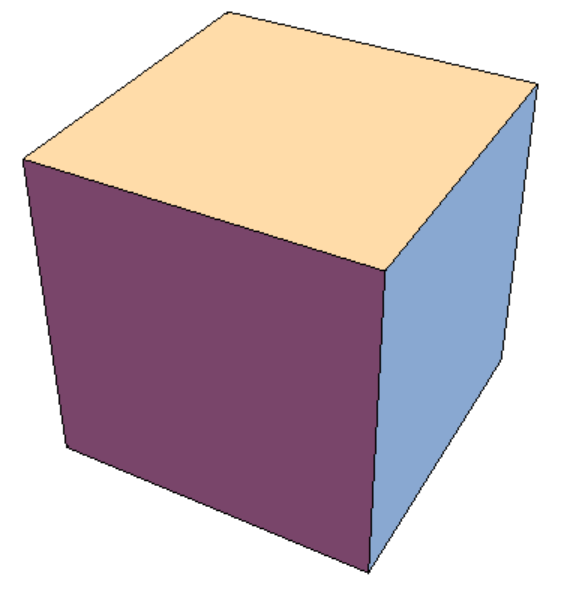
\includegraphics[width=0.3\textwidth]{figures/cube}
	\caption{A figure caption beneath the figure for description of the depicted concept which sometimes can be very long}
	\label{ft_fig_firstfig}
\end{figure}

In \autoref{ft_fig_firstfig}, for example, a PNG image is depicted (compiled with pdflatex). Alternatively, EPS figures can be embedded if dvips and ps2pdf compilation is used. All figures are listed in the list of figures with the command \imp{listoffigures}.

\section{Tables}

Data can be presented in tables, e.g., as shown in \autoref{ft_tab_ex}.

\begin{table}[!h]
	\centering
	\begin{tabular}{l|cl}
	\hline \hline
	
		& Property 1
		& Property 2\\ \hline
	Criterion 1
		& 764
		& 23546 \\
	Criterion 2
		& 3
		& 34 \\
	\hline \hline
	\end{tabular}
	\caption{Exemplary table}
	\label{ft_tab_ex}
\end{table}

Sometimes very long tables must be presented which may also go over pages. For this cases the packages \imp{longtable} is useful, as used in 

\begin{center}
\begin{longtable}{l|l|l}

% \baselinestretch{1.5}

 \hline \hline
 $i^3$ & $2i^3$ & $3i^3$ \bigstrut \\ \hline
 \endfirsthead
 
 \multicolumn{3}{c}{\tablename\ \thetable{} -- information message on top} \\
 \hline
 $i^3$ & $2i^3$ & $3i^3$ \bigstrut \\ \hline 
 \endhead
 
 \hline
 \multicolumn{3}{c}{Foot information} \\ \hline
 \endfoot
 
 \hline \hline
 \caption{Long Table}
 \label{lt}
 \endlastfoot
 
 1 & 2 & 3 \\
 8 & 16 & 24 \\
 27 & 54 & 81 \\
 64 & 128 & 192 \\
 125 & 250 & 375 \\
 216 & 432 & 648 \\
 343 & 686 & 1029 \\
 512 & 1024 & 1536 \\
 729 & 1458 & 2187 \\
 1000 & 2000 & 3000 \\
 1331 & 2662 & 3993 \\
 1728 & 3456 & 5184 \\
 2197 & 4394 & 6591 \\
 2744 & 5488 & 8232 \\
 3375 & 6750 & 10125 \\
 4096 & 8192 & 12288 \\
 4913 & 9826 & 14739 \\
 5832 & 11664 & 17496 \\
 6859 & 13718 & 20577 \\
 8000 & 16000 & 24000 \\
 9261 & 18522 & 27783 \\
 10648 & 21296 & 31944 \\
 12167 & 24334 & 36501 \\
 13824 & 27648 & 41472 \\
 15625 & 31250 & 46875 \\
 17576 & 35152 & 52728 \\
 19683 & 39366 & 59049 \\
 21952 & 43904 & 65856 \\
 24389 & 48778 & 73167 \\
 27000 & 54000 & 81000 \\
 29791 & 59582 & 89373 \\
 32768 & 65536 & 98304 \\
 35937 & 71874 & 107811 \\
 39304 & 78608 & 117912 \\
 42875 & 85750 & 128625 \\
 46656 & 93312 & 139968 \\
 50653 & 101306 & 151959 \\
 54872 & 109744 & 164616 \\
 59319 & 118638 & 177957 \\
 64000 & 128000 & 192000 \\
 68921 & 137842 & 206763 \\
 74088 & 148176 & 222264 \\
 79507 & 159014 & 238521 \\
 85184 & 170368 & 255552 \\
 91125 & 182250 & 273375 \\
 97336 & 194672 & 292008 \\
 103823 & 207646 & 311469 \\
 110592 & 221184 & 331776 \\
 117649 & 235298 & 352947 \\
 125000 & 250000 & 375000 \\
\end{longtable}
\end{center}

All tables are listed with \imp{listoftables}.

\section{Enumerate and itemize}

If important sequential points are to presented the environment \imp{enumerate} can be used as follows:
\begin{enumerate}
\item
	Some important stuff
\item
	More stuff
\end{enumerate}
With the package \imp{enumerate} some options can be used, e.g.,
\begin{enumerate}[a)]
\item
	Some important stuff
\item
	More stuff
\end{enumerate}
or 
\begin{enumerate}[~~~1)]
\item
	Some important stuff
\item
	More stuff
\end{enumerate}

Alternatively, point can be just presented without any enumeration with the environment \imp{itemize}
\begin{itemize}
\item
	Some important stuff
\item
	More stuff
\end{itemize}

%\chapter{Appendix, footnotes, todos and index}
\begin{appendix}

\chapter{Just an example appendix}
\label{app_ex1}

%\section{Appendix}
%
%For many reasons some concept may be important for the document but too long for the main text. In this kind of cases these concept can be presented with the environment \imp{appendix} in appendices, e.g., as in \autoref{app_ex1} and \autoref{app_ex2}.

%%%%%%%%%%%%%%%%%%%%%%%%%%%%%%%%%%%%%%%%%%%%%%%%%%%%%%%%%%%
%%%%%%%%%%%%%%%%%%%%%%%%%%%%%%%%%%%%%%%%%%%%%%%%%%%%%%%%%%%

%\section{Footnotes}
%
%You may want to give additional information to some points\footnote{Bla bla} in the text\footnote{Blu blup}.

%%%%%%%%%%%%%%%%%%%%%%%%%%%%%%%%%%%%%%%%%%%%%%%%%%%%%%%%%%%
%%%%%%%%%%%%%%%%%%%%%%%%%%%%%%%%%%%%%%%%%%%%%%%%%%%%%%%%%%%

%\section{Todos}
%
%With the package \imp{todonotes} comments\todo{like this one}\ pointing to their place can be embedded into the text. These comments are veeeery useful if you are writing something for the first time or are working on a draft. The todos can be listed with \imp{listoftodos} where you want it to appear in order to see what is unfinished or needs some more work.

%%%%%%%%%%%%%%%%%%%%%%%%%%%%%%%%%%%%%%%%%%%%%%%%%%%%%%%%%%%
%%%%%%%%%%%%%%%%%%%%%%%%%%%%%%%%%%%%%%%%%%%%%%%%%%%%%%%%%%%

%\section{Index}
%
%If the document is very long, it may be very useful for a lot of readers to have an index for searching key words and certain concepts (Crtl+F is usually very helpful in PDFs but not always the best solution). For this, the  package \imp{makeidx}, the commands \imp{makeindex} and \imp{printindex} and the compiling option \imp{make index} are needed. You may want to index different words like heterogeneous materials\index{Heterogeneous materials}, effective properties\index{Effective properties} and homogenization\index{Homogenization}.


%\begin{appendix}

%\chapter{Just an example appendix}
%\label{app_ex1}

%\section{Bla blup}
%
%Sme stuff
%\begin{equation}
%	f(x) = \int_{\Omega} g(x) dx \ .
%\end{equation}

%\chapter{Another example}
%\label{app_ex2}

%\section{More stuff}

%Bla bla.

\end{appendix}

%\bibliographystyle{plain}
\bibliographystyle{abbrvnat}
\bibliography{literature/library}

\listoffigures
\listoftables

\printindex

\end{document}
